\hypertarget{funnel-metadynamics-tutorial}{%
\label{funnel-metadynamics-tutorial}}
\hypertarget{Introduction}{%
\subsubsection{Introduction}\label{Introduction}}

Funnel metadynamics (fun-metaD) is a molecular dynamics-based method
that calculates the absolute binding free energy (ABFE) between a small
organic ligand and a protein. It uses an enhanced sampling method called
metadynamics, that speeds up the molecular processes of interest by
periodically adding small amounts of bias. To best separate the bound
and unbound phases, as well as increase the rate of convergence, the
exploration of the ligand in 3D space is limited by funnel-shaped
restraints.

This tutorial paper will describe how to setup and analyse fun-metaD
simulations. The main paper that explains what fun-metaD is by
\href{https://www.pnas.org/content/110/16/6358}{Limogelli \emph{et al}
2013} but in this tutorial I will describe the
\href{https://www.ncbi.nlm.nih.gov/pmc/articles/PMC7467642/}{Rhys
\emph{et al} 2020} and
\href{https://pubs.acs.org/doi/10.1021/acs.jcim.6b00772}{Saleh \emph{et
al} 2017} implementation. The main difference between the two
implementations is the functional form of the funnel restraints: the
original fun-metaD relied on a cone and a cylinder joined to make a
funnel using a step function, while the new implementation uses a single
sigmoid function. The Limogelli implementation also requires the protein
to be realigned with a reference structure to keep the funnel strictly
in place over the binding site, which hurts the performance. The
implementation I will describe here allows the funnel to move with the
protein.

Up to now, one of the biggest drawbacks to using fun-metaD for
large-scale absolute binding free energy (ABFE) calculations was the
difficulty in setting up the simulations. It's hard to know where the
funnel should be defined, how big it needs to be, what each of the
sigmoid function parameters should be set to, along with the chore of
writting PLUMED files, where each protein and ligand system will have
slightly different atom IDs.

BioSimSpace has made this easier, automatically defining the funnel
using abstract features of the protein cavity, assigning the relevant
atom IDs, suggesting reasonable default funnel parameters and allowing
the visualisation of the funnel restraints inside a Jupyter Notebook.
All this leads to a quicker setup and much faster automation of large
ABFE screening campaigns.

By the end of this tutorial you should know: 1. The basics of what
fun-metaD does. 2. How to setup fun-metaD simulations and how to
visualise the funnel restraints. 3. How to analyse the results of a
fun-metaD simulation.

\hypertarget{the-theory}{%
\subsubsection{The Theory}\label{the-theory}}

Metadynamics is an enhanced sampling method that biases a simulation
along a chosen set of reaction coordinates, or as MetaD practitioners
call them, collective variables (CVs). This bias is deposited at defined
time intervals and takes the shape of a Gaussian potential.
Investigation of drug binding should involve at least one CV, distance
from the drug molecule to the protein, where the distance between them
can be biased, causing the drug to unbind. However, that single distance
is degenerate, meaning many different configurations of the drug in 3D
space will not be described by that single distance. It also involves
the exploration of a very large volume, hindering convergence.

Fun-metaD gets around both of these problems, restricting the
exploration by using funnel-shaped restraints and reducing degeneracy by
using two CVs - `projection' and `extent'. See Figure \ref{fig:funnel}.

\begin{figure}[htp]
\includegraphics[width=\linewidth]{02_funnel_metad/figures/figure1.jpeg}
\caption{Visualised funnel restraints.}
\label{fig:funnel}
\end{figure}

The restraints that limit the pp.ext CV follow a sigmoid function:

\begin{equation}
S = h\left(\frac{1}{1+b^{b(i-x)}}\right) + f
\end{equation}

where, S is the maximal distance from the axis, at pp.proj = i, h is the
`wall\_width', f is the `wall\_buffer', b is the `beta\_cent' (the
steepness at the inflection point), x is the `s\_cent' (the inflection
point as a value of pp.proj). The exploration along the pp.proj is
limited by the `lower\_wall' and `upper\_wall' parameters. The funnel's
radius at the narrow end is equal to `wall\_buffer'. `P0' and `Px' are
the points that define the funnel's vector. From now on I'll refer to
them as p0 and p1, respectively.

Clearly, there is still some degeneracy in the CVs - the plane
perpendicular to the projection axis is a one dimensional representation of a two dimensional space. However, this is a good compromise between having sufficient accuracy for describing the binding of a
ligand and the tolerable simulation slowdown of using only two CVs.

In ordered to have a good separation between the bound and unbound phases for the ABFE estimations, the funnel needs to point `out', with the narrow end in the solvent,
and away from any protein residues. BSS funnel assignment code does this pretty well. Most of the vectors it picks for defining the p0 and p1 points are good enough for an unobstructed exit path for the ligand. It is still a good idea to check, especially for new protein systems, by
having a look using the funnel visualisation functionality within BSS.

In terms of deciding on how big the radius of funnel should be, it varies on a case-by-case basis.
In general, the funnel will need to be smaller than it seems necessary. The metadynamics code tracks the exploration of the center of mass of the ligand, so the volume that the small molecule will explore is much bigger than it looks intuitively. There is usually only one binding site and the funnel should enclose only it, excluding other protein
features, by setting a small `wall\_width'. This really helps with
convergence by preventing the drug molecule from exploring irrelevant
regions in the free energy surface (FES). Other funnel parameters do not influence matters
that much and the default settings will suffice in most situations.

\hypertarget{visualising-restraints}{%
\subsubsection{Visualising funnel restraints}\label{Visualising the funnel restraints}}

Before we go on to setting up the metadynamics simulation, we can quickly check the funnel restraints using BSS. Load the fully solvated HSP90 protein-ligand system (PDBID:2WI2) and the suggested funnel restraints:

\begin{python}
import BioSimSpace as BSS

# Load the system.
system = BSS.IO.readMolecules(
            ["input_files/solvated.prm7",
             "input_files/solvated.rst7"])

# Create the funnel parameters.
p0, p1 = BSS.Metadynamics.CollectiveVariable.makeFunnel(
            system)

# Define the collective variable.
funnel_cv = BSS.Metadynamics.CollectiveVariable.Funnel(
            p0, p1)

# Create a view.
view = BSS.Metadynamics.CollectiveVariable.viewFunnel(
            system, funnel_cv)

view.system()

\end{python}

Figure \ref{fig:fun-hsp90} below is what you should see in your Jupyter Notebook. 

\begin{figure}[htp]
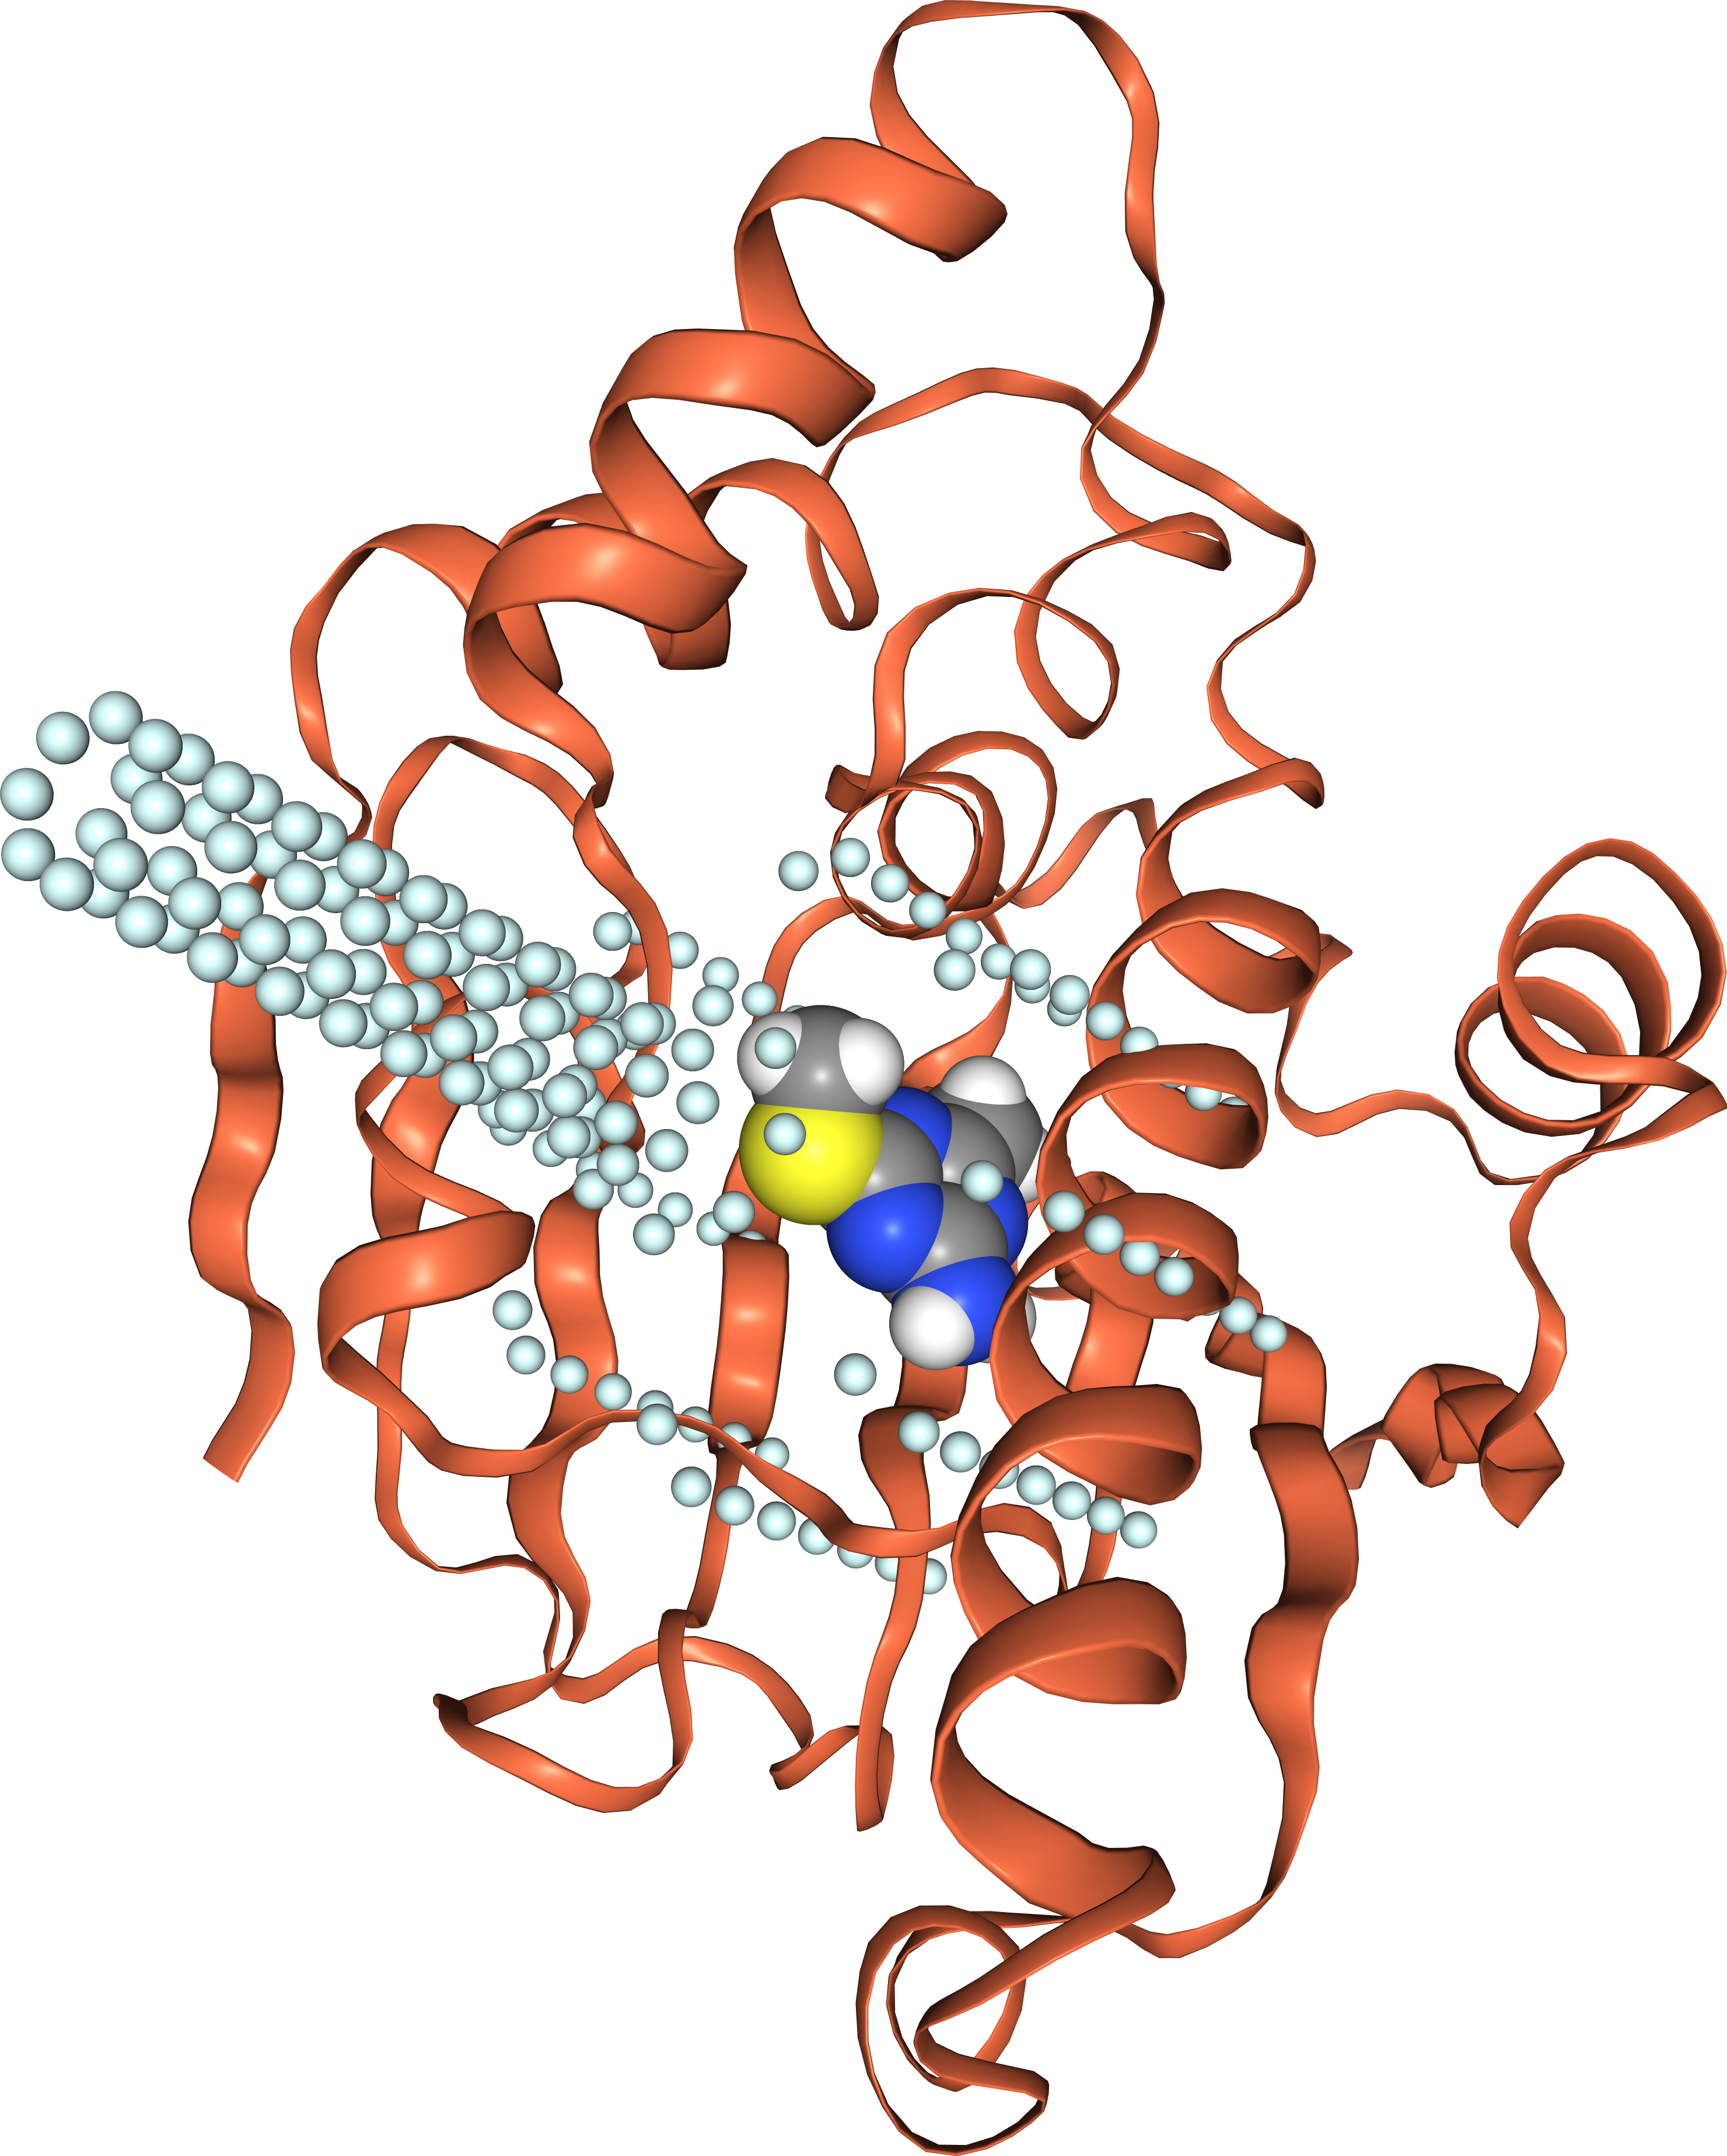
\includegraphics[width=\linewidth]{02_funnel_metad/figures/fun-hsp90.png}
% \caption{Visualised funnel restraints.}
\label{fig:fun-hsp90}
\end{figure}

The funnel vector is clearly pointing out into the solvent, with no protein residues blocking the way. The default radius is sufficient to encompass the binding site, excluding rest of the protein.

\hypertarget{setting-up-the-simulation}{%
\subsubsection{Setting up the simulation}\label{setting-up-the-simulation}}

For this part, open the \texttt{02\_bss-fun-metad-tutorial.ipynb}
notebook.

\hypertarget{analysis}{%
\subsubsection{Analysing fun-metaD simulations}\label{analysis}}

Open the \texttt{03\_bss-fun-metad-analysis.ipynb} notebook.
